% homework template
\documentclass[a4paper,11pt]{article}

%package declarations:
%geometry:set the geometry of page
%ragged2e: left/right justify
%fancyhdr: header/footers
\usepackage{geometry}
\usepackage{ragged2e}
\usepackage{fancyhdr}
\usepackage{amsmath,amssymb,amsthm,graphicx}
\usepackage{algorithm}
\usepackage{algpseudocode}
\usepackage{wrapfig}
\usepackage{epsfig}
\usepackage{float}

%redefine maketitle
%http://tex.stackexchange.com/questions/85343/left-align-abstract-title-and-authors
\renewcommand{\maketitle}{%
	
	\Large
 	\textbf{CS 204, Spring 2017}
 	\hfill
 	SDN Assignment Report
 	\par
 	
	\Large
	Abhishek Kumar SRIVASTAVA
	\hfill
	\normalsize
	\today
 	\par
 	Student ID: 861307778
 	\par
 	
 	%plagiarism statement
 	%\begin{center}

 	%\vspace{.2in}
 	
 	%\textit{I certify that this submission represents my own original work }
 	%\par
	%\vspace{.2in}
	%\makebox[2.4in]{\hrulefill}
	%\par

 	%\end{center}
 	
 	\hrulefill
 	\par \vspace{2ex}
 	}


%since using the assignment class, set the geometry
\geometry{total={210mm,297mm},
	left=25mm,right=25mm,%
	bindingoffset=0mm, top=20mm,bottom=20mm}

%set headers and footers
\pagestyle{fancy}
\fancyhf{}
\fancyhead[LE,RO]{\textbf{CS 204:} SDN-Assignment}
\fancyhead[RE,LO]{Abhishek Kumar Srivastava}
\fancyfoot[CE,CO]{\leftmark}
\fancyfoot[LE,RO]{\thepage}

%some custom commands, taken from stanford template
\newtheoremstyle{quest}{\topsep}{\topsep}{}{}{\bfseries}{}{ }{\thmname{#1}\thmnote{ #3}.}
\theoremstyle{quest}
\newtheorem*{definition}{Definition}
\newtheorem*{theorem}{Theorem}
\newtheorem*{question}{Question}
\newtheorem*{exercise}{Exercise}
\newtheorem*{challengeproblem}{Challenge Problem}
\newenvironment{solution}[2][Solution]{\begin{trivlist}
		\item[\hskip \labelsep {\bfseries #1}\hskip \labelsep {\bfseries #2.}]}{\end{trivlist}}

\begin{document}\thispagestyle{empty}
	
\maketitle

\begin{solution}
\textbf{Setup Screenshots}:
\begin{figure}[h]
	\centering
	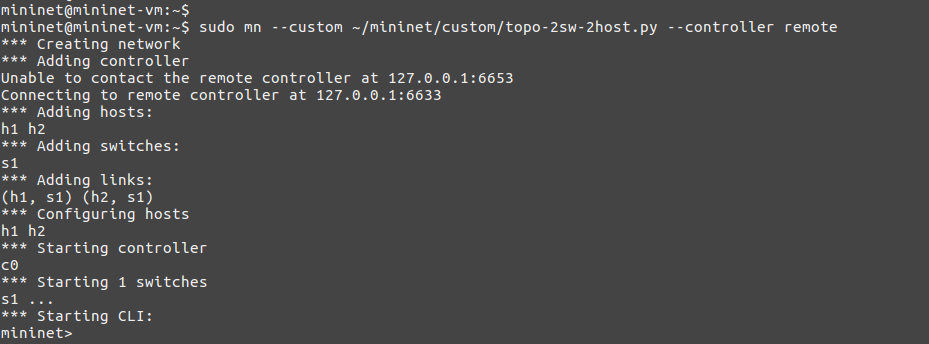
\epsfig{file=sdn_0_0.png, height=2.3in, width=6in}
	\caption{Setting up	a test topology that connects to the controller and switches.}
\end{figure}	
\begin{figure}[h]
	\centering
	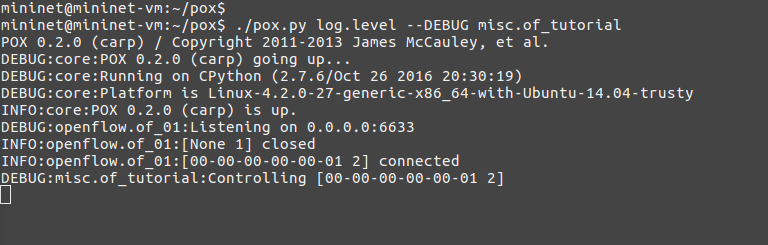
\epsfig{file=sdn_0_1.png, height=1.95in, width=6in}
	\caption{Running the controller which connects to switches as seen in the output.}
\end{figure}

\begin{figure}[h]
	\centering
	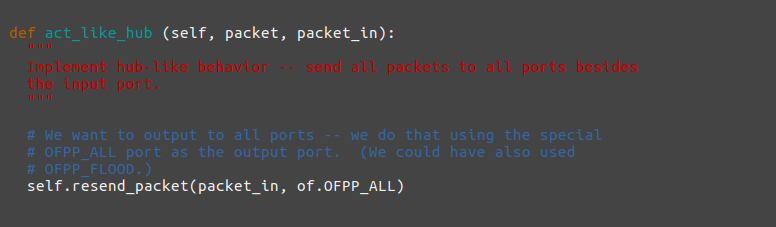
\epsfig{file=sdn_20_5.png, height=1.75in, width=6in}
	\caption{``of\_tutorial'' act as dumb switch(hub) and floods packets to all port except the input port.}
\end{figure}

\begin{figure}[h]
	\centering
	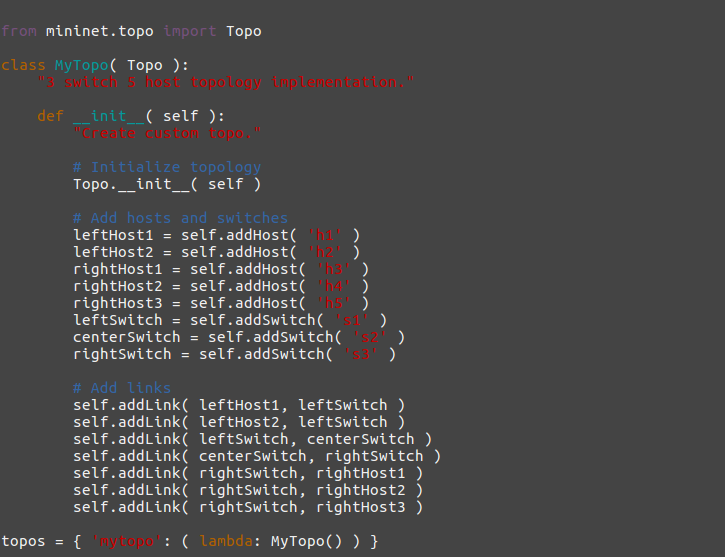
\epsfig{file=sdn_20_0.png, height=4.75in, width=6in}
	\caption{Code to create topology of 5hosts \& 3 switches and add links as specified in the problem: ``topo-3sw-5host''.}
\end{figure}

\begin{figure}[h]
	\centering
	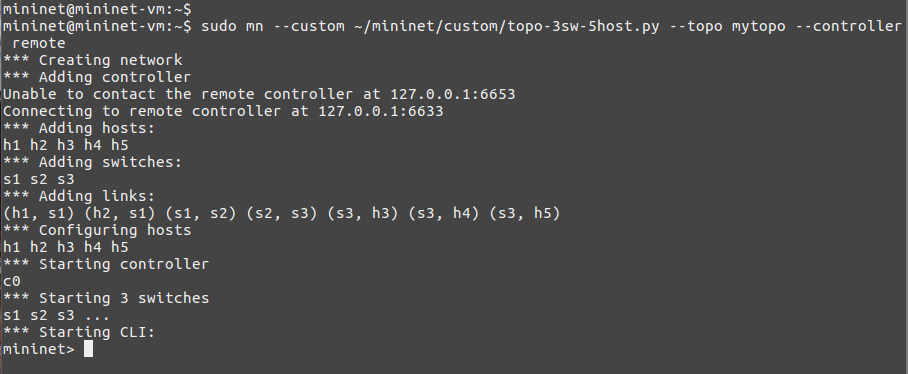
\epsfig{file=sdn_1.png, height=3in, width=6in}
	\caption{Running ``topo-3sw-5host'' network topology.}
\end{figure}
\begin{figure}[h]
	\centering
	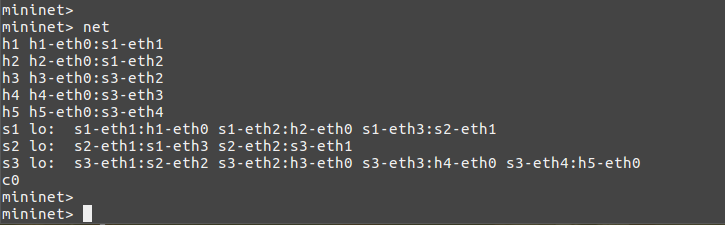
\epsfig{file=sdn_9.png, height=2.25in, width=6in}
	\caption{Showing connections for the ``topo-3sw-5host'' topology.}
\end{figure}
\begin{figure}[h]
	\centering
	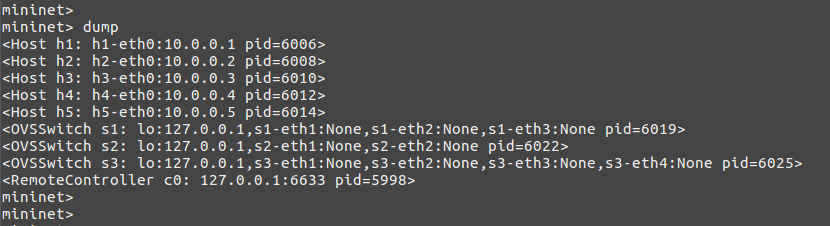
\epsfig{file=sdn_8.png, height=1.75in, width=6in}
	\caption{Ip Addresses of switches and hosts.}
\end{figure}	
\begin{figure}[h]
	\centering
	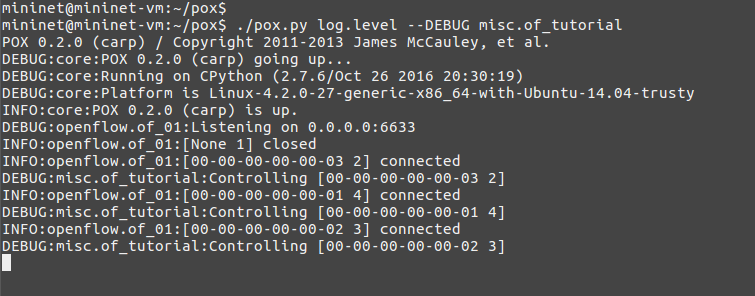
\epsfig{file=sdn_a.png, height=2.5in, width=6in}
	\caption{Output of running remote controller ``of\_tutorial''. All 3 switches able to connect to the controller.}
\end{figure}
	
%Solution A:
\begin{figure}[h]
	\centering
	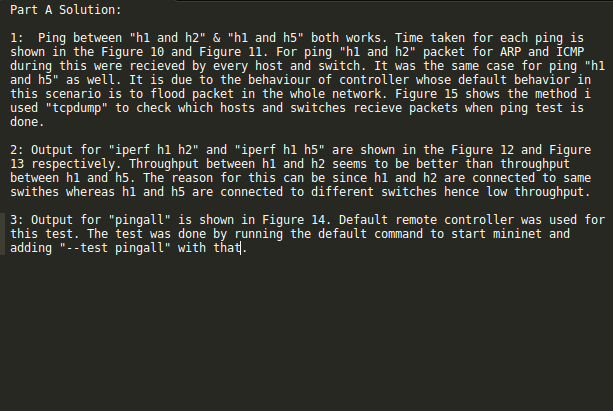
\epsfig{file=sdn_ans_a.png, height=4.25in, width=6in}
	\caption{Solution A.}
\end{figure}
\begin{figure}[h]
	\centering
	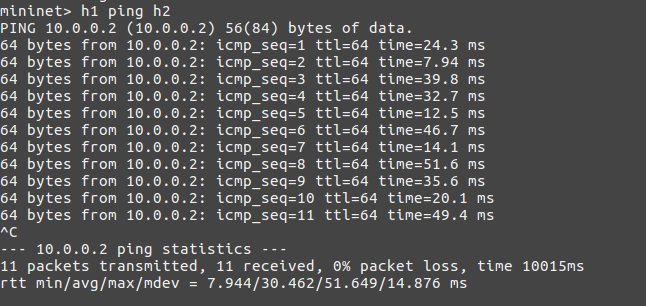
\epsfig{file=sdn_3.png, height=2.75in, width=6in}
	\caption{Output of ``h1 ping h2'' command for default behavior of controller.}
\end{figure}
\begin{figure}[h]
	\centering
	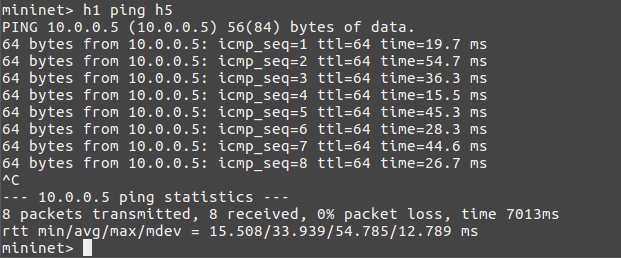
\epsfig{file=sdn_4.png, height=2.75in, width=6in}
	\caption{Output of ``h1 ping h5'' command for default behavior of controller.}
\end{figure}
\begin{figure}[h]
	\centering
	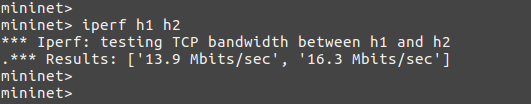
\epsfig{file=sdn_5.png, height=1.25in, width=6in}
	\caption{Output of ``iperf h1 h2'' command for default behavior of controller.}
\end{figure}
\begin{figure}[h]
	\centering
	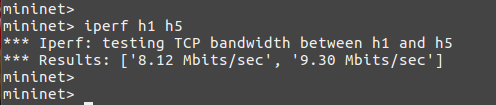
\epsfig{file=sdn_6.png, height=1.25in, width=6in}
	\caption{Output of ``iperf h1 h5'' command for default behavior of controller.}
\end{figure}
\begin{figure}[h]
	\centering
	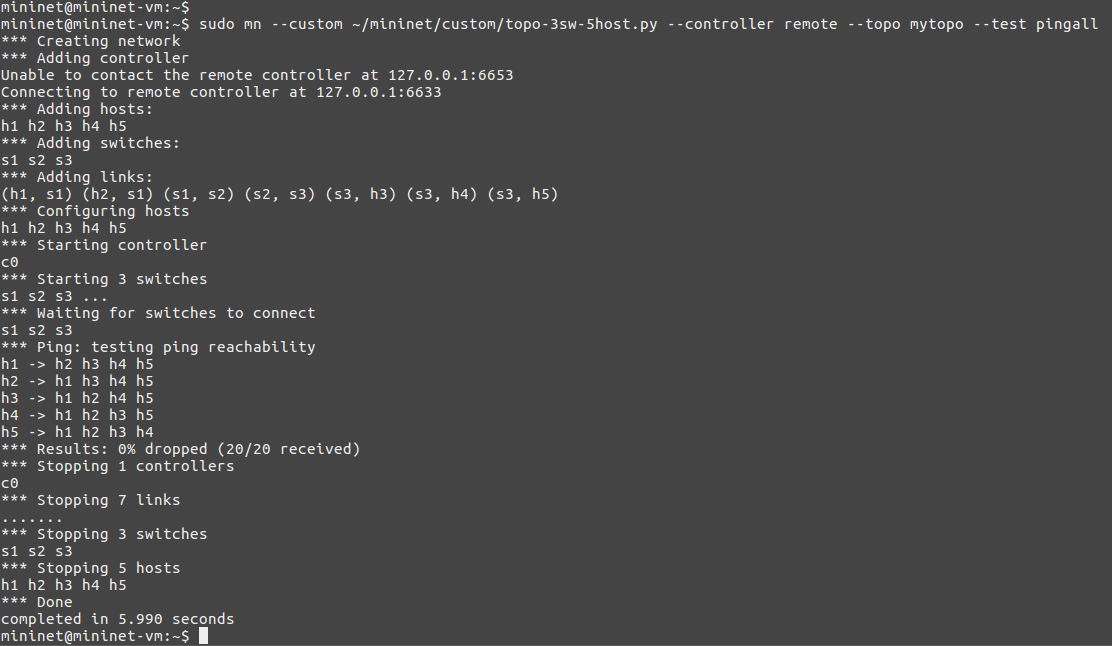
\epsfig{file=sdn_7_1.png, height=4.25in, width=7in}
	\caption{``Pingall'' test for default behavior of controller.}
\end{figure}
\begin{figure}[h]
	\centering
	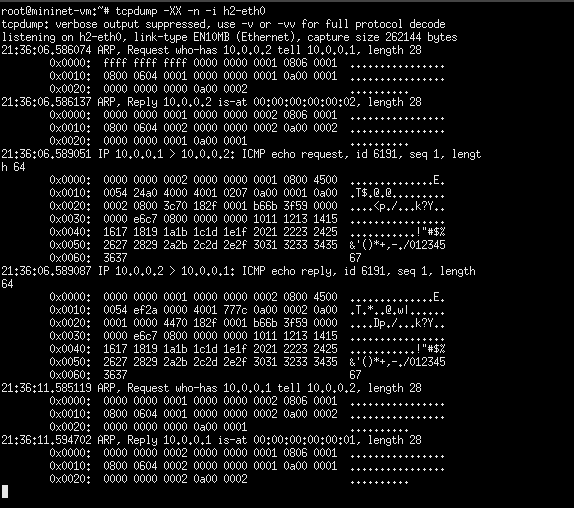
\epsfig{file=sdn_12.png, height=4.5in, width=6in}
	\caption{``tcpdump'' used to check which switches and hosts are receiving packets.}
\end{figure}

%Solution B:
\begin{figure}[h]
	\centering
	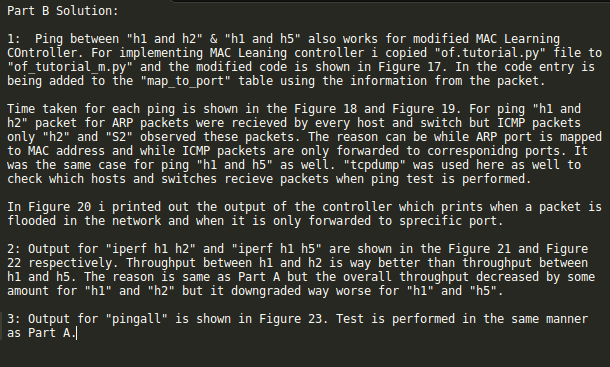
\epsfig{file=sdn_ans_b.png, height=3.75in, width=6in}
	\caption{Solution B.}
\end{figure}
\begin{figure}[h]
	\centering
	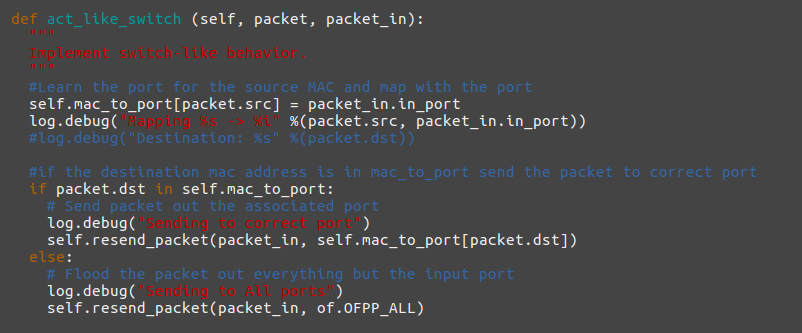
\epsfig{file=sdn_20_1.png, height=3in, width=6in}
	\caption{Code for MAC learning. MAC address is mapped to the port and packet is only flooded only if port is not found in map table.}
\end{figure}
\begin{figure}[h]
	\centering
	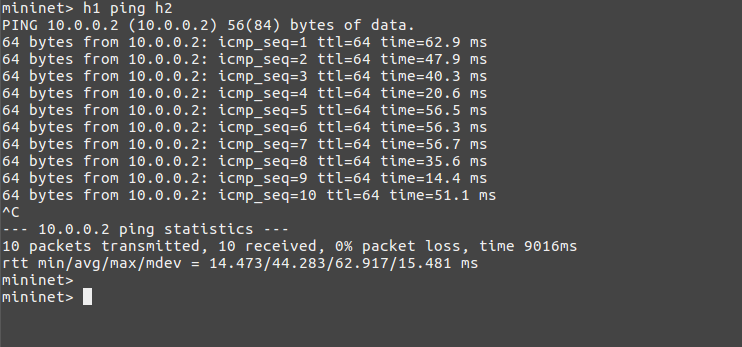
\epsfig{file=sdn_14_1.png, height=3in, width=6in}
	\caption{Output for ``h1 ping h2'' command for MAC learning controller.}
\end{figure}
\begin{figure}[h]
	\centering
	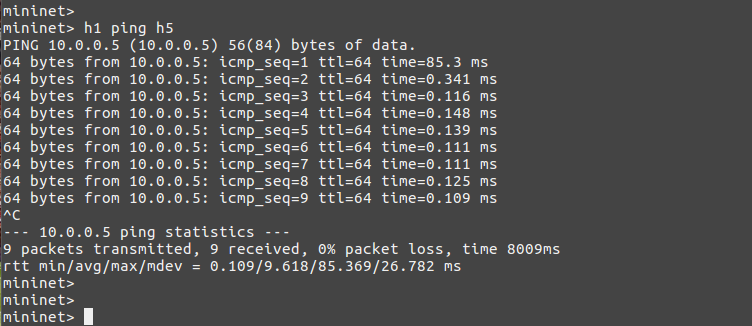
\epsfig{file=sdn_16_3.png, height=3in, width=6in}
	\caption{Output for ``h1 ping h5'' command for MAC learning controller.}
\end{figure}
\begin{figure}[h]
	\centering
	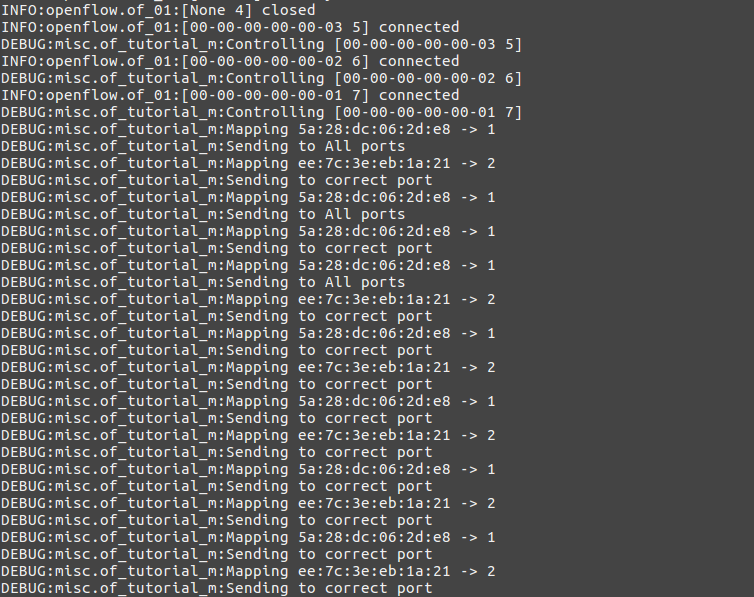
\epsfig{file=sdn_14_2.png, height=5in, width=6in}
	\caption{Output of MAC learning controller which shows which packet is being forwarded to correct port and which one is flooded out.}
\end{figure}
\begin{figure}[h]
	\centering
	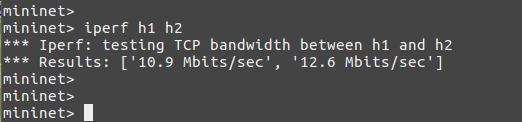
\epsfig{file=sdn_14_B2_1.png, height=1.5in, width=6in}
	\caption{Throughput of h1 and h2 by running ``iperf h1 h2'' command.}
\end{figure}
\begin{figure}[h]
	\centering
	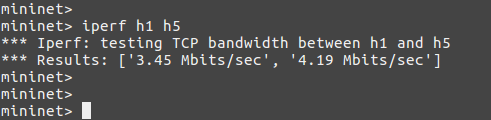
\epsfig{file=sdn_14_B2__2.png, height=1.5in, width=6in}
	\caption{Throughput of h1 and h2 by running ``iperf h1 h2'' command.}
\end{figure}
\begin{figure}[h]
	\centering
	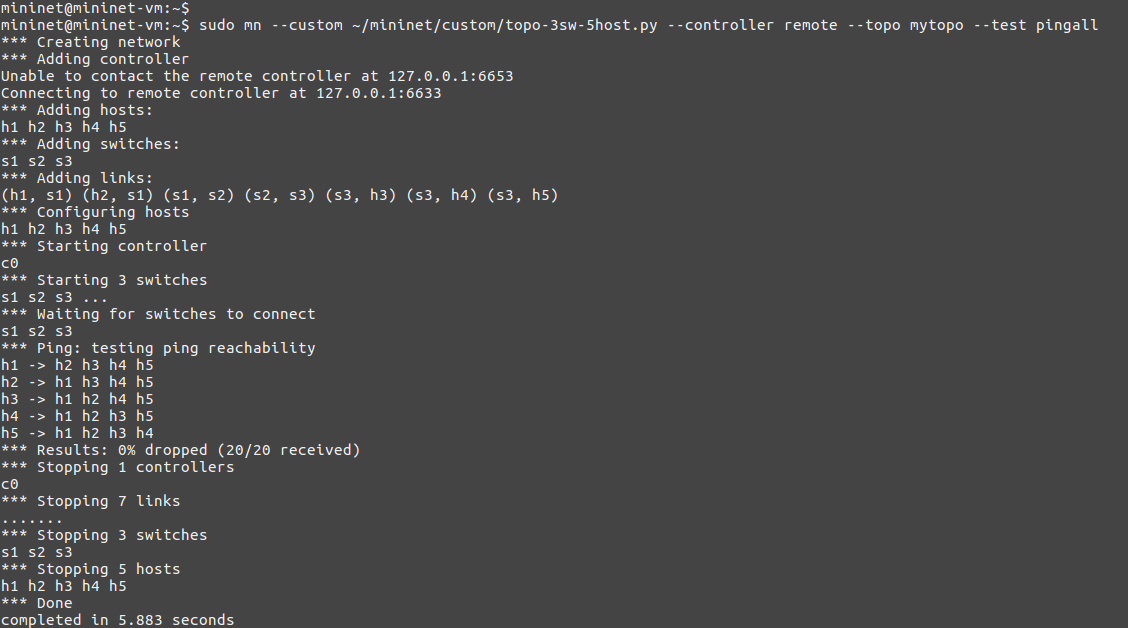
\epsfig{file=sdn_15_1.png, height=4.25in, width=7in}
	\caption{Output of ``pingall'' command test for MAC learning controller.}
\end{figure}

%Solution C:
\begin{figure}[h]
	\centering
	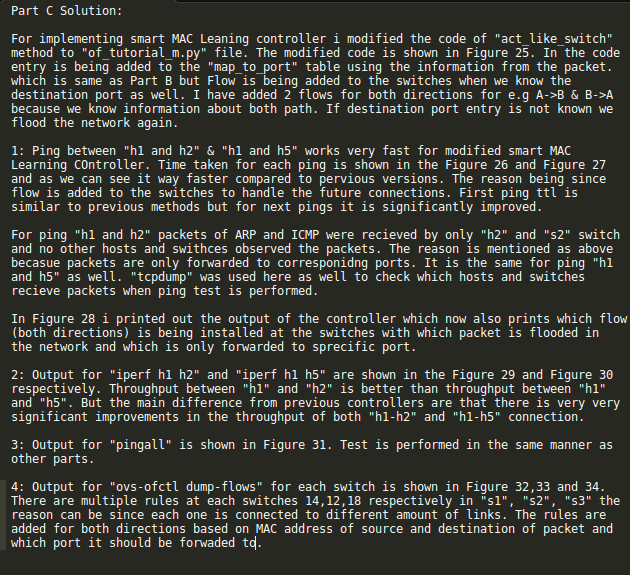
\epsfig{file=sdn_ans_c.png, height=5in, width=6in}
	\caption{Solution C.}
\end{figure}
\begin{figure}[h]
	\centering
	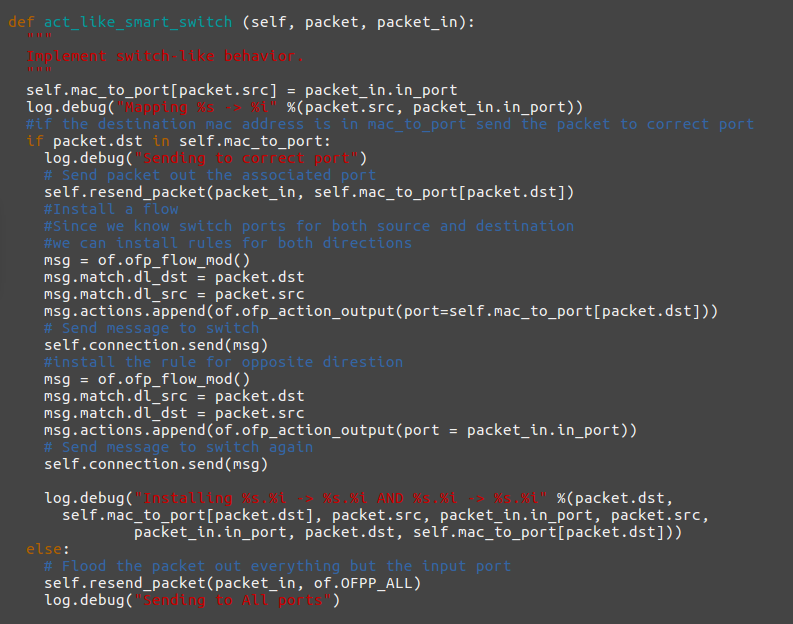
\epsfig{file=sdn_20_2.png, height=5in, width=6in}
	\caption{Code for Smart MAC learning. MAC address is mapped to the port and packet is only flooded only if port is not found in map table.}
\end{figure}
\begin{figure}[h]
	\centering
	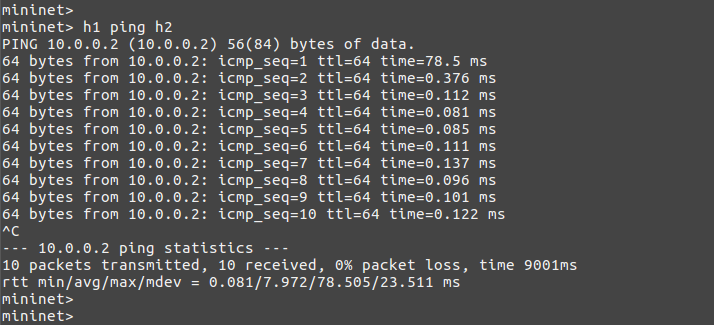
\epsfig{file=sdn_16_1_1.png, height=3in, width=6in}
	\caption{Output for ``h1 ping h2'' command for Smart MAC learning controller.}
\end{figure}
\begin{figure}[h]
	\centering
	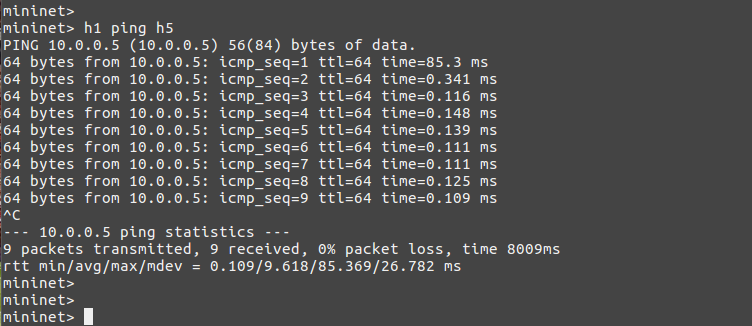
\epsfig{file=sdn_16_3.png, height=3in, width=6in}
	\caption{Output for ``h1 ping h5'' command for Smart MAC learning controller.}
\end{figure}
\begin{figure}[h]
	\centering
	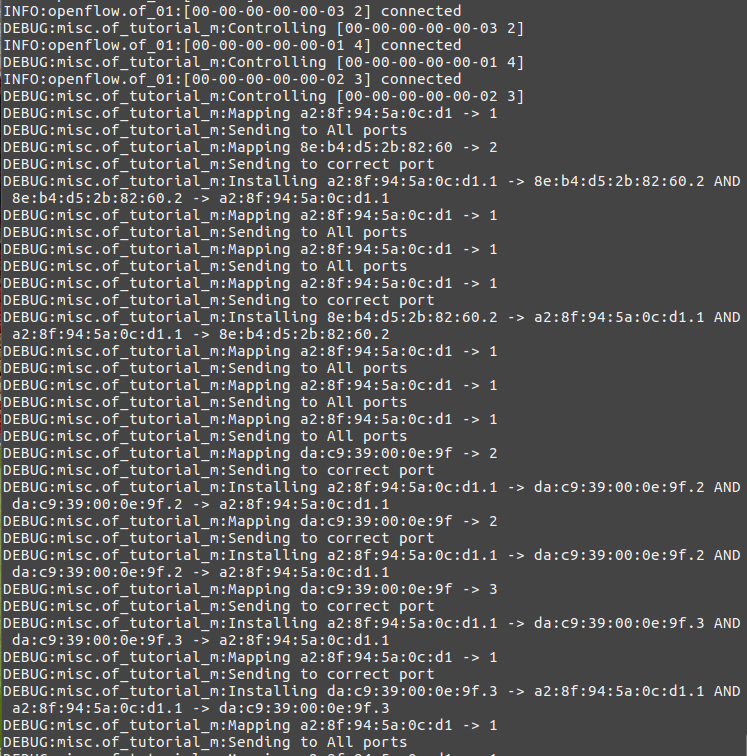
\epsfig{file=sdn_18_2.png, height=6in, width=6in}
	\caption{Output of MAC learning controller which shows which packet is being forwarded to correct port and which one is flooded out.}
\end{figure}
\begin{figure}[h]
	\centering
	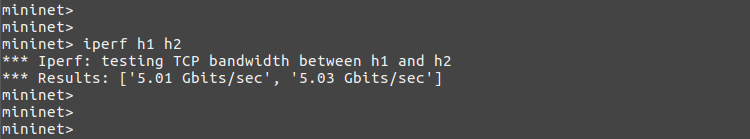
\epsfig{file=sdn_17_C2_1.png, height=1.4in, width=6in}
	\caption{Throughput of h1 and h2 by running ``iperf h1 h2'' command for Smart MAC learning controller.}
\end{figure}
\begin{figure}[h]
	\centering
	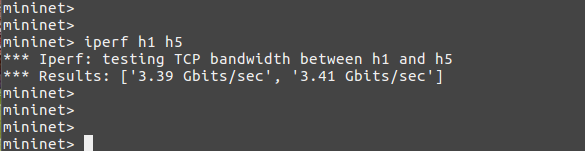
\epsfig{file=sdn_17_C2_2.png, height=1.5in, width=6in}
	\caption{Throughput of h1 and h2 by running ``iperf h1 h2'' command for Smart MAC learning controller.}
\end{figure}
\begin{figure}[h]
	\centering
	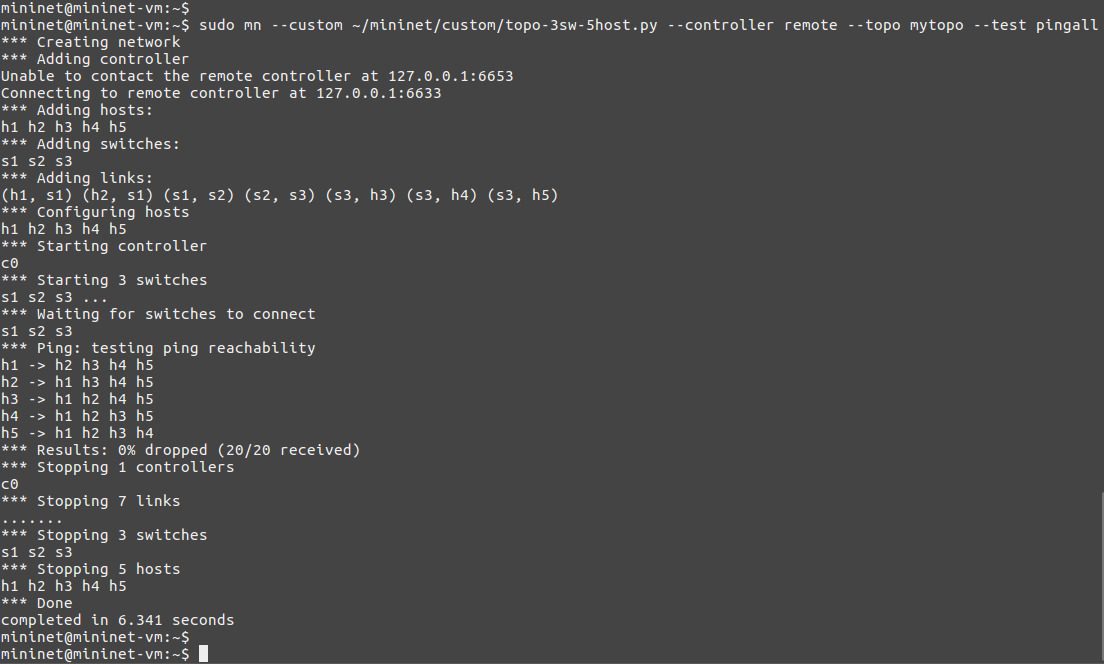
\epsfig{file=sdn_18_3.png, height=4.35in, width=6in}
	\caption{Output of ``pingall'' command test for Smart MAC learning controller.}
\end{figure}
\begin{figure}[h]
	\centering
	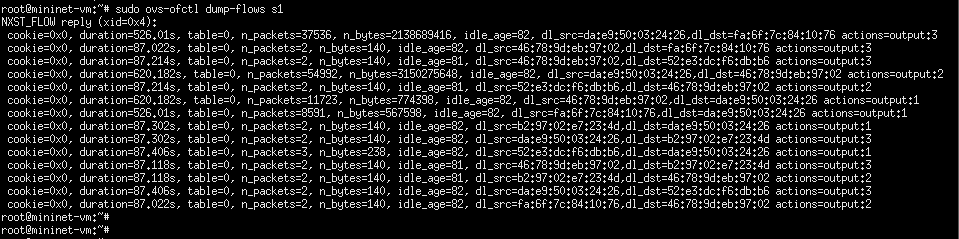
\epsfig{file=sdn_19_1.png, height=1.75in, width=6in}
	\caption{Output of ``ovs-ofctl dump-flows'' command at S1 switch for Smart MAC learning controller.}
\end{figure}
\begin{figure}[h]
	\centering
	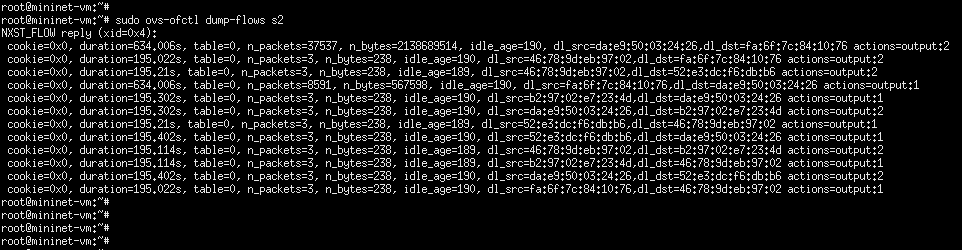
\epsfig{file=sdn_19_2.png, height=1.75in, width=6in}
	\caption{Output of ``ovs-ofctl dump-flows'' command at S2 switch for Smart MAC learning controller.}
\end{figure}
\begin{figure}[h]
	\centering
	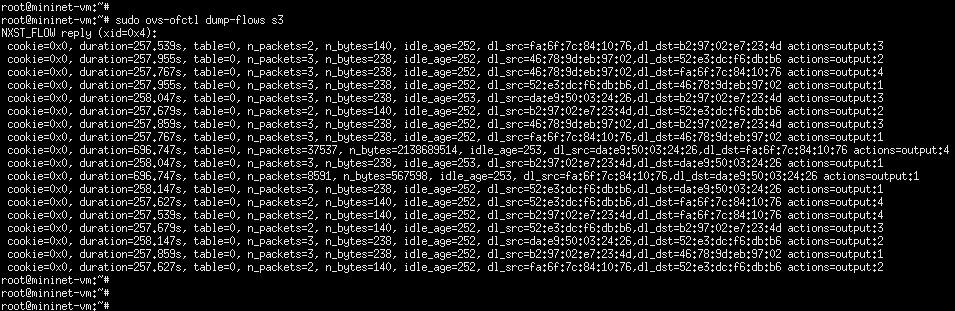
\epsfig{file=sdn_19_3.png, height=2in, width=7in}
	\caption{Output of ``ovs-ofctl dump-flows'' command at S3 switch for Smart MAC learning controller.}
\end{figure}

%Solution D:
\begin{figure}[h]
	\centering
	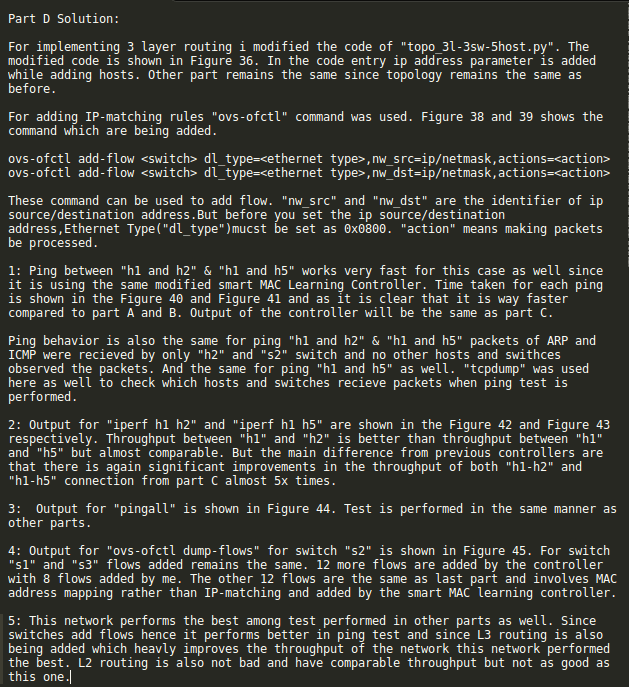
\epsfig{file=sdn_ans_d.png, height=5.75in, width=6in}
	\caption{Solution D.}
\end{figure}
\begin{figure}[h]
	\centering
	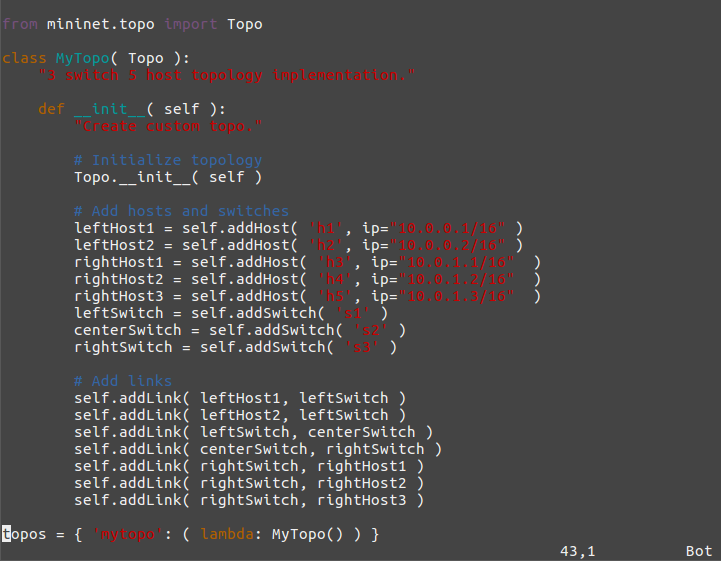
\epsfig{file=sdn_23.png, height=4.75in, width=6in}
	\caption{Code for Smart MAC learning. MAC address is mapped to the port and packet is only flooded only if port is not found in map table.}
\end{figure}
\begin{figure}[h]
	\centering
	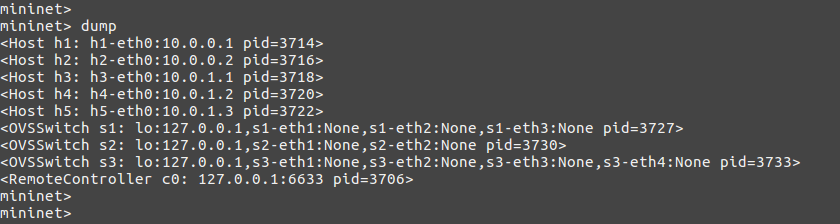
\epsfig{file=sdn_23_6.png, height=2.1in, width=6in}
	\caption{Network topology created with specified IP/Subnets in the assignment.}
\end{figure}
\begin{figure}[h]
	\centering
	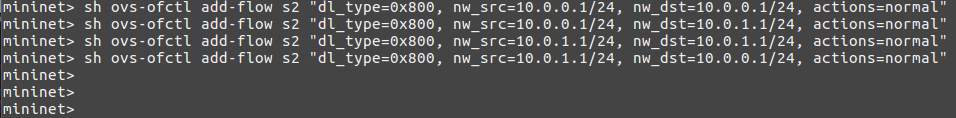
\epsfig{file=sdn_21_1.png, height=1.1in, width=6.5in}
	\caption{IP matching Rule addition}
\end{figure}
\begin{figure}[h]
	\centering
	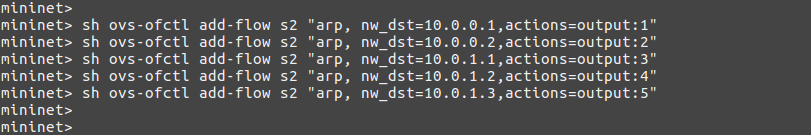
\epsfig{file=sdn_21_2.png, height=1.25in, width=6in}
	\caption{IP matching Rule addition for specific address.}
\end{figure}
\begin{figure}[h]
	\centering
	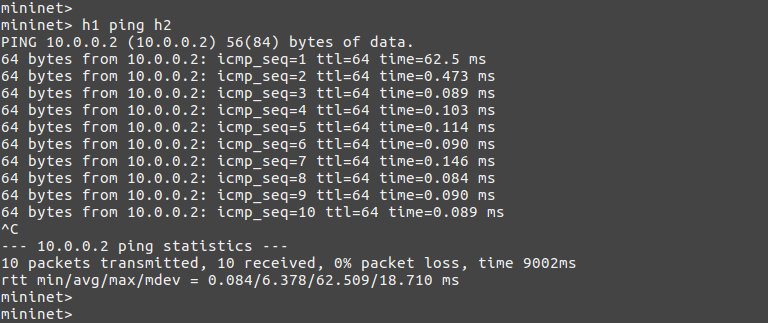
\epsfig{file=sdn_21_5.png, height=3in, width=6in}
	\caption{Output for ``h1 ping h2'' command for Smart MAC learning controller.}
\end{figure}
\begin{figure}[h]
	\centering
	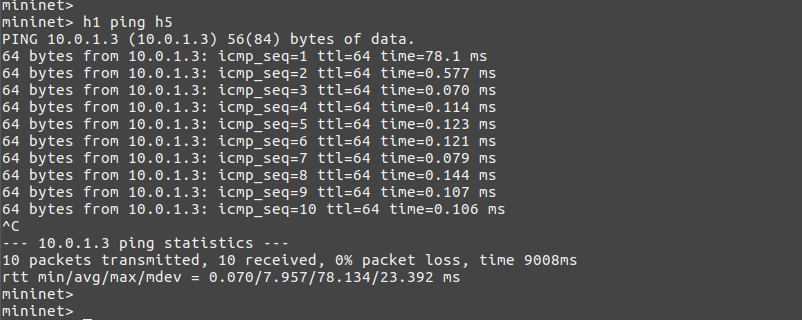
\epsfig{file=sdn_21_6.png, height=3in, width=6in}
	\caption{Output for ``h1 ping h5'' command for Smart MAC learning controller.}
\end{figure}
\begin{figure}[h]
	\centering
	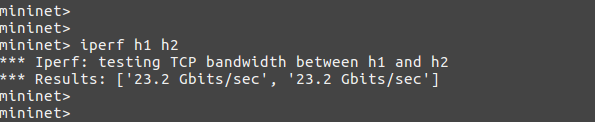
\epsfig{file=sdn_22_D_2_1.png, height=1.4in, width=6in}
	\caption{Throughput of h1 and h2 by running ``iperf h1 h2'' command for Smart MAC learning controller.}
\end{figure}
\begin{figure}[h]
	\centering
	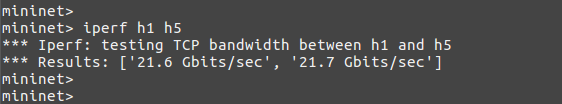
\epsfig{file=sdn_22_D_2_2.png, height=1.4in, width=6in}
	\caption{Throughput of h1 and h2 by running ``iperf h1 h2'' command for Smart MAC learning controller.}
\end{figure}
\begin{figure}[h]
	\centering
	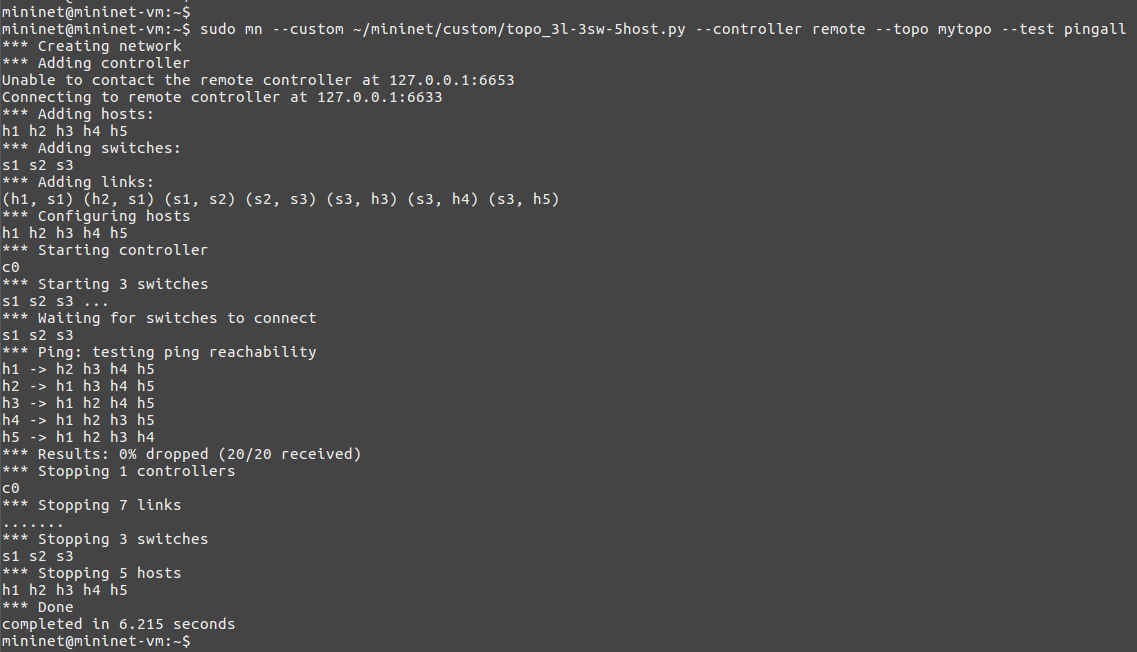
\epsfig{file=sdn_23_5.png, height=4.35in, width=6in}
	\caption{Output of ``pingall'' command test for Smart MAC learning controller.}
\end{figure}
\begin{figure}[h]
	\centering
	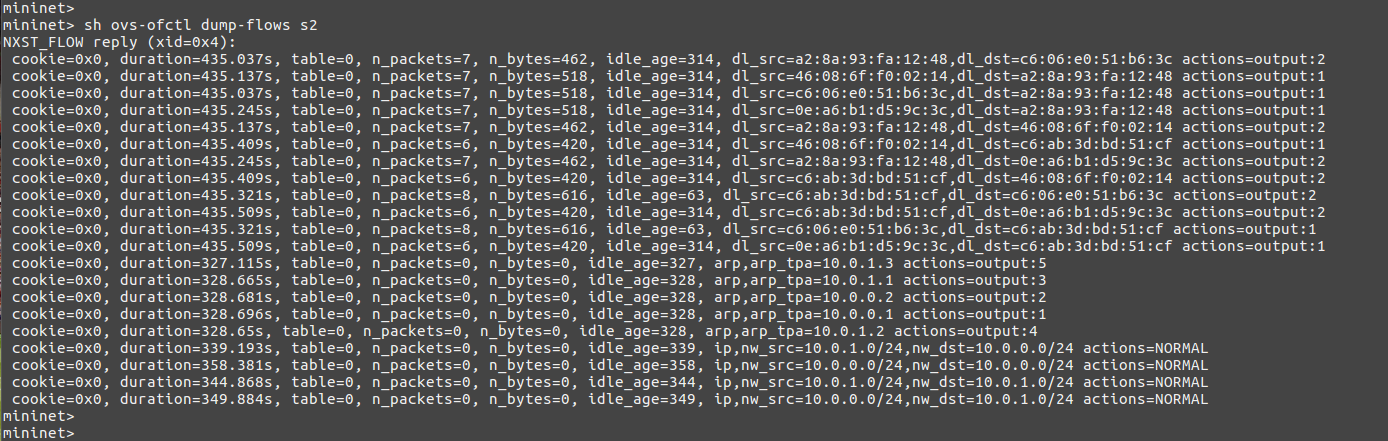
\epsfig{file=sdn_21_4.png, height=2.5in, width=6in}
	\caption{Output of ``ovs-ofctl dump-flows'' command at S2 switch for Smart MAC learning controller.}
\end{figure}
\end{solution}
\end{document}